\documentclass[12pt]{article}
\usepackage{amssymb}
\usepackage[UTF8]{ctex}
\usepackage{geometry}
\usepackage{units}
\usepackage{pifont}
\geometry{
	a4paper,
	total={150mm,237mm},
	left=30mm,
	top=27mm,
	}
\usepackage{amsmath}
\usepackage{enumerate}
\usepackage{lipsum}
\usepackage{graphicx}
\usepackage{hyperref}
\usepackage{indentfirst}
\usepackage[graphicx]{realboxes}
\usepackage{booktabs}
\usepackage{cases}
\usepackage{subfig}  
\usepackage{float}
\usepackage{pythonhighlight}

\setlength{\parindent}{2em}
\title{HW10}
\author{姓名:陈锐林,学号:21307130148}

\begin{document}
\maketitle
\begin{large}
    \noindent Question1:\par
\end{large}
线程的顺序可能会改变。\\
\begin{large}
    Question2:\par
\end{large}
加上-d标志后,也会看到执行顺序的不同;可能会看到死锁的发生。如把-l提高到1000,经过多次试验都不会死锁;但是提高到100000.就经常会死锁。\\
\begin{large}
    Question3:\par
\end{large}
显而易见的,随着-n的增大,即线程数的增加,死锁会发生得更频繁。能保证不发生死锁的n只有0和1了,因为再大的2在Q2中,只要循环数多了一样会死锁。\\
\begin{large}
    Question4:\par
\end{large}
(1)避免死锁是因为采用了全局的顺序判断,对dst和src进行判断,觉得lock的顺序。(2)特殊情况是因为不能对一个锁尝试上锁两次,会死锁。\\
\begin{large}
    Question5:\par
\end{large}
(1)由下图看出来,"./vector-global-order -t -n 2 -l 100000 -d"命令,用时为0.05s。(2)而随着线程数和循环数的增大,所用时也会增加;从这几组数据来看,增加线程数的提升是非线性的、增加循环数的提升是线性的。
\begin{figure}[H]
    \centering
    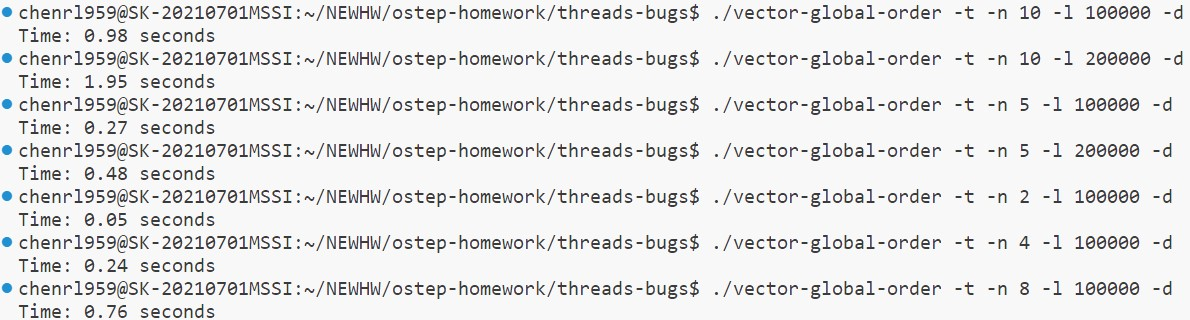
\includegraphics[height=4cm]{hw10-1.jpg}
\end{figure}
\newpage
\begin{large}
    \noindent Question6:\par
\end{large}
(1)用时会减短。(2)我预测表现会更好,因为不同的线程不再需要一直等待两个vector。下图也表明如此:
\begin{figure}[H]
    \centering
    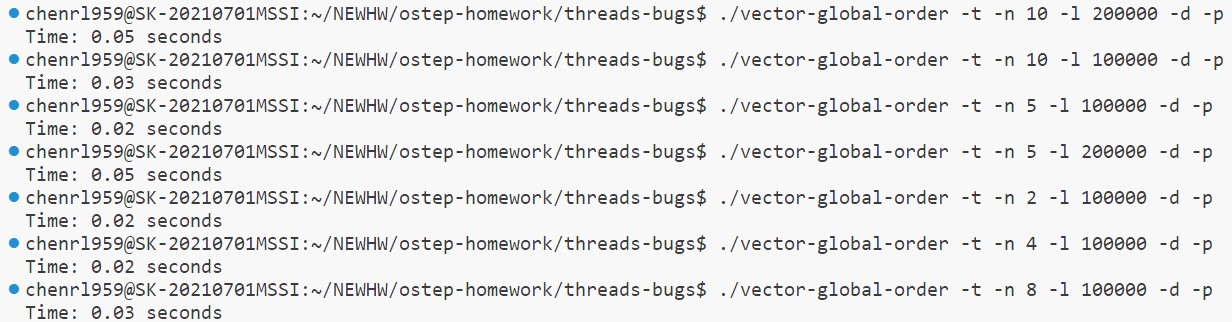
\includegraphics[height=4cm]{hw10-2.jpg}
\end{figure}
\begin{large}
    \noindent Question7:\par
\end{large}
(1)这里的pthread\_mutex\_trylock是没有必要的;它在这里不会进入休眠,而是持续跳转到top,这是浪费时间的。(2)如果采用-p标签,能看到Retries都是0,用时更少;但如果不用-p,能看到表现并没有前几问的好。(3)(不-p情况下)Retries个数是呈指数上涨的。
\begin{figure}[H]
    \centering
    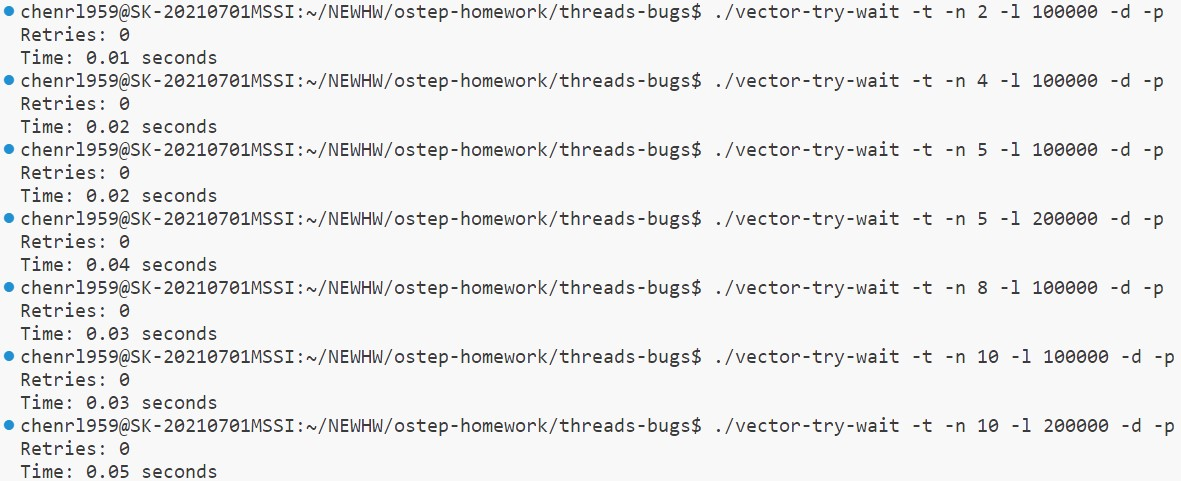
\includegraphics[height=5.5cm]{hw10-3.jpg}
\end{figure}
\begin{figure}[H]
    \centering
    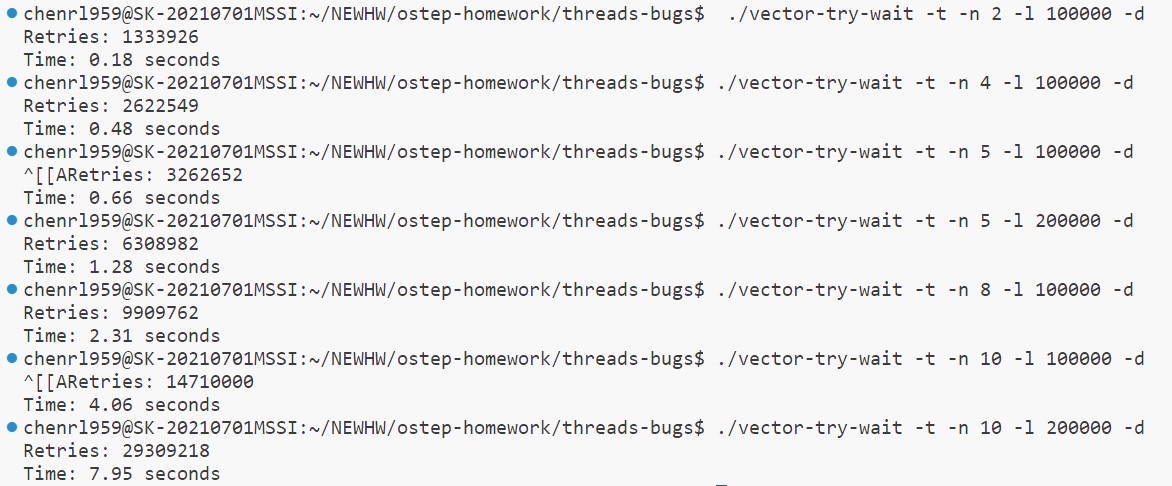
\includegraphics[height=5.5cm]{hw10-4.jpg}
\end{figure}
\newpage
\begin{large}
    \noindent Question8:\par
\end{large}
(1)主要问题在于,全局锁的存在导致,即使两个线程在不同向量上操作,也要等待。(2)取两个情况对-p和不带-p进行测试,能看到;带-p的vector-avoid-hold-and-wait是比较慢的,但是不带-p的情况下,还是会比vecotr-global-order略快(或差不多),比vector-try-wait快得多。
\begin{figure}[H]
    \centering
    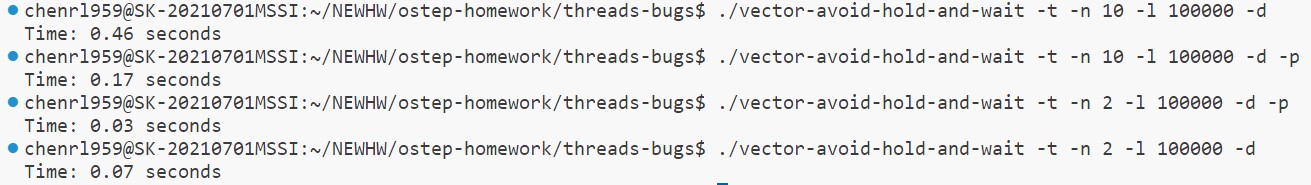
\includegraphics[height=2cm]{hw10-5.jpg}
\end{figure}
\begin{large}
    \noindent Question9:\par
\end{large}
首先这个版本没有调用任何关于lock的函数,而是使用了fetch\_and\_add来解决问题。但是这个版本在语义上应该是一样的,asm volatile("lock; xaddl \%\%eax, \%2;")表明了fetch\_and\_add的内部实现仍然是用到了锁相关的知识,可能只是更底层而已。\\
\begin{large}
    Question10:\par
\end{large}
能看到这个版本倒也不是那么快,带-p和不带都比vector-avoid-hold-and-wait慢;和vector-global-order和vector-try-wait比,也只有不带-p是快。
\begin{figure}[H]
    \centering
    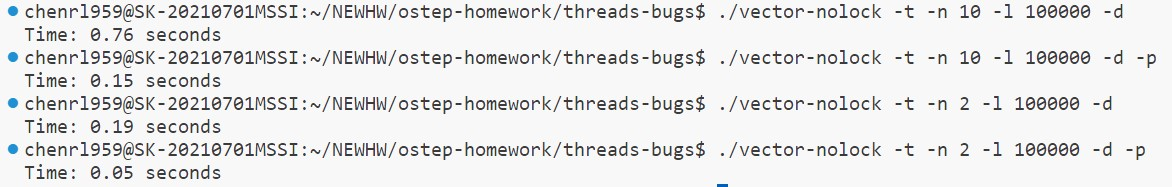
\includegraphics[height=2cm]{hw10-6.jpg}
\end{figure}
\end{document}